\section{Experiments}
We test the Bayesian Quadrature Riemannian Laplace approximation using a small toy classification data set and the UCI Wine data set. The tou dataset consist of a single input dimension, and three classes as seen in figure \ref{fig:}. We compare the Bayesian Quadrature with the normal Riemannian Laplace approximation, a vanilla Laplace approximation and the MAP solution. 

For the Bayesian Quadrature model, the predictive distribution is approximated by taking Monte Carlo sampling where we take $1000$ parameter samples from the quadrature approximation and calculate mean and prediction intervals from this.


\begin{figure}[h]
    \centering
    \subfloat[Integrand values]{
        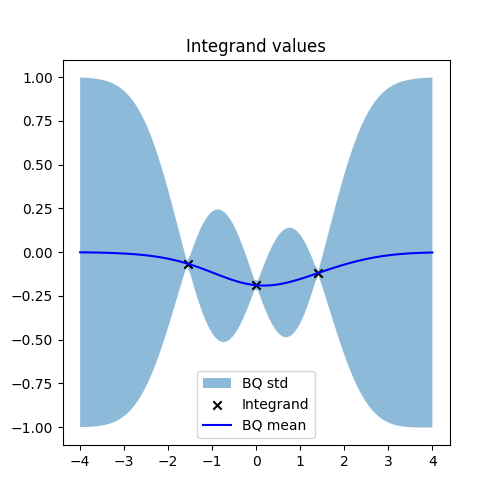
\includegraphics[width=.31\linewidth]{report/figures/UFA_BQ_integrand_vals_1d.png}
        \label{fig:UFA_BQ_integrand_vals_1d}
    }
    \hfill
    \subfloat[Integrand values and measure]{
        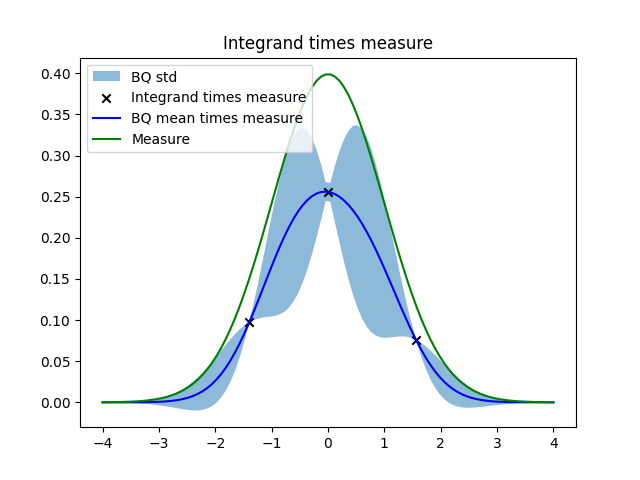
\includegraphics[width=.31\linewidth]{report/figures/UFA_BQ_integrand_vals_measure_1d.png}
        \label{fig:UFA_BQ_integrand_vals_measure_1d}
    }
    \hfill
    \subfloat[Bayesian Quadrature Riemannian Laplace approximation for UFA]{
        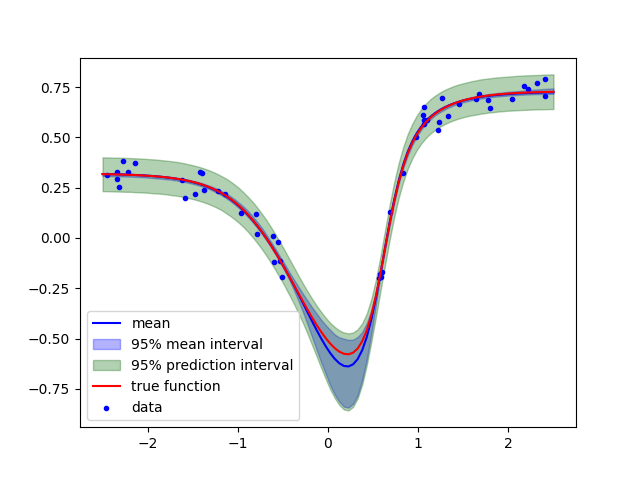
\includegraphics[width=.31\linewidth]{report/figures/UFA_riemannian_BQ_subspace_rank2.png}
        \label{fig:UFA_BQ_variance}
    }
    \caption{Bayesian Quadrature}
    \label{fig:bayesian_quadrature1}
\end{figure}
